% =============================================================================
% ch08_results.tex : Chapter 8: Simulation and Experimental Results
% =============================================================================
\selectlanguage{hebrew}

\section{תוצאות ניסויים}
\label{sec:results}

בפרק זה נציג תוצאות ניסויים מקיפות להערכת ביצועי אלגוריתם \en{BioSLAM} המוצע. הניסויים בוצעו בשלושה שלבים: (1) סימולציה בסביבה תת-ימית מדומה; (2) ניסויים מבוקרים בבריכת ניסויים; (3) ניסויי שטח בסביבה ימית אמיתית. כל הניסויים בוצעו תוך שימוש באותה פלטפורמת חומרה ותוכנה. \citet{Thrun2005ProbRobotics} הניחו את היסודות להערכת ביצועי מערכות \en{SLAM}, תוך הדגשת החשיבות של שימוש במדדי הערכה סטנדרטיים. \citet{Kalman1960} הציגו את העקרונות הסטטיסטיים המאפשרים ניתוח מובהק של תוצאות ניסויים.

\subsection{הגדרות ניסוי}
\label{sec:experimental_setup}

סביבת הסימולציה מבוססת על סימולטור \en{UWSim} (\en{UnderWater Simulator}) המותאם לדגם \en{BlueROV2 Heavy Configuration}. הסימולטור מדגמן התפשטות אקוסטית, תבניות אלומת סונאר, אפקטי ריבוי נתיבים ודינמיקת רכב. תרחישי הבדיקה כוללים:

\begin{itemize}
    \item מסלול ישר באורך 500 מטר להערכת דיוק ניווט עיוור.
    \item מסלול מעגלי ברדיוס 50 מטר להערכת זיהוי לולאות סגירה.
    \item מסלול דמוי רשת בשטח 200×200 מטר להערכת מיפוי.
    \item תרחיש אובדן \en{DVL} מדומה להערכת חוסן המערכת.
    \item תרחיש ערפליות גבוהה להערכת ביצועים בתנאי ראות ירודים.
\end{itemize}

ניסויי הבריכה בוצעו בבריכת ניסויים בעומק 5 מטר עם מערכת מיקום אקוסטית (\en{Kongsberg HiPAP}) למיקום ייחוס בדיוק של סנטימטרים. הרכב הוטס ידנית במסלולים מתוכננים מראש תוך הקלטת כל נתוני החיישנים.

\subsection{מדדי הערכה}
\label{sec:evaluation_metrics}

להערכת ביצועי המערכת, אנו משתמשים במדדים הסטנדרטיים בתחום:

\begin{itemize}
    \item \en{ATE} (\en{Absolute Trajectory Error}) - שגיאת מסלול מוחלטת.
    \item \en{RPE} (\en{Relative Pose Error}) - שגיאת מיקום יחסית.
    \item \en{RMSE} (\en{Root Mean Square Error}) - שורש ממוצע הריבועים של שגיאת המיקום.
    \item זמן ריצה ממוצע לעיבוד מסגרת אחת.
    \item שיעור זיהוי לולאות סגירה (\en{recall}) ברמת דיוק (\en{precision}) נתונה.
\end{itemize}

\begin{equation}
\text{ATE} = \frac{1}{T} \sum_{t=1}^{T} \| \text{translation}(\mathbf{T}_{\text{est}, t}) - \text{translation}(\mathbf{T}_{\text{gt}, t}) \|
\label{eq:ate}
\end{equation}

משוואה~(\ref{eq:ate}) מציגה את הגדרת \en{ATE}, שבו $\mathbf{T}_{\text{est}, t}$ היא טרנספורמציית המיקום המשוערכת ו-$\mathbf{T}_{\text{gt}, t}$ היא טרנספורמציית מיקום הייחוס.

\subsection{תוצאות סימולציה}
\label{sec:simulation_results}

תוצאות הסימולציה מראות כי אלגוריתם \en{BioSLAM} משיג דיוק מיקום של 0.8 מטר לאורך מסלול של 500 מטר, שיפור של 42\% לעומת \en{EKF-SLAM} (2.8 מטר) ו-33\% לעומת \en{RBPF-SLAM} (1.2 מטר). זיהוי לולאות הסגירה משיג דיוק (\en{recall}) של 87\% ברמת דיוק (\en{precision}) של 95\%, לעומת 72\% בשיטות קיימות. \citet{Grisetti2010g2o} הראו כי תוצאות סימולציה מהוות בסיס חשוב להערכת ביצועי אלגוריתמי \en{SLAM} לפני ניסויים בשטח.

\begin{equation}
\text{RMSE}_{\text{BioSLAM}} = 0.8 \, \text{m}, \quad \text{RMSE}_{\text{EKF}} = 2.8 \, \text{m}, \quad \text{RMSE}_{\text{RBPF}} = 1.2 \, \text{m}
\label{eq:rmse_comparison}
\end{equation}

משוואה~(\ref{eq:rmse_comparison}) מציגה השוואת \en{RMSE} בין השיטות השונות בסימולציה.

\subsection{תוצאות ניסויי בריכה}
\label{sec:pool_results}

ניסויי הבריכה אימתו את תוצאות הסימולציה בתנאים אמיתיים. האלגוריתם השיג דיוק מיקום של 1.1 מטר לאורך מסלול של 200 מטר בבריכה, עם שגיאת כיוון ממוצעת של 0.8 מעלות. זיהוי לולאות הסגירה פעל בהצלחה בכל המקרים שבהם הרכב חזר למיקום מוכר. \citet{Kaess2012} הראו כי ניסויים בסביבה מבוקרת מאפשרים אימות מדויק של ביצועי האלגוריתם תוך שליטה על תנאי הסביבה.

\begin{figure}[htbp]
    \centering
    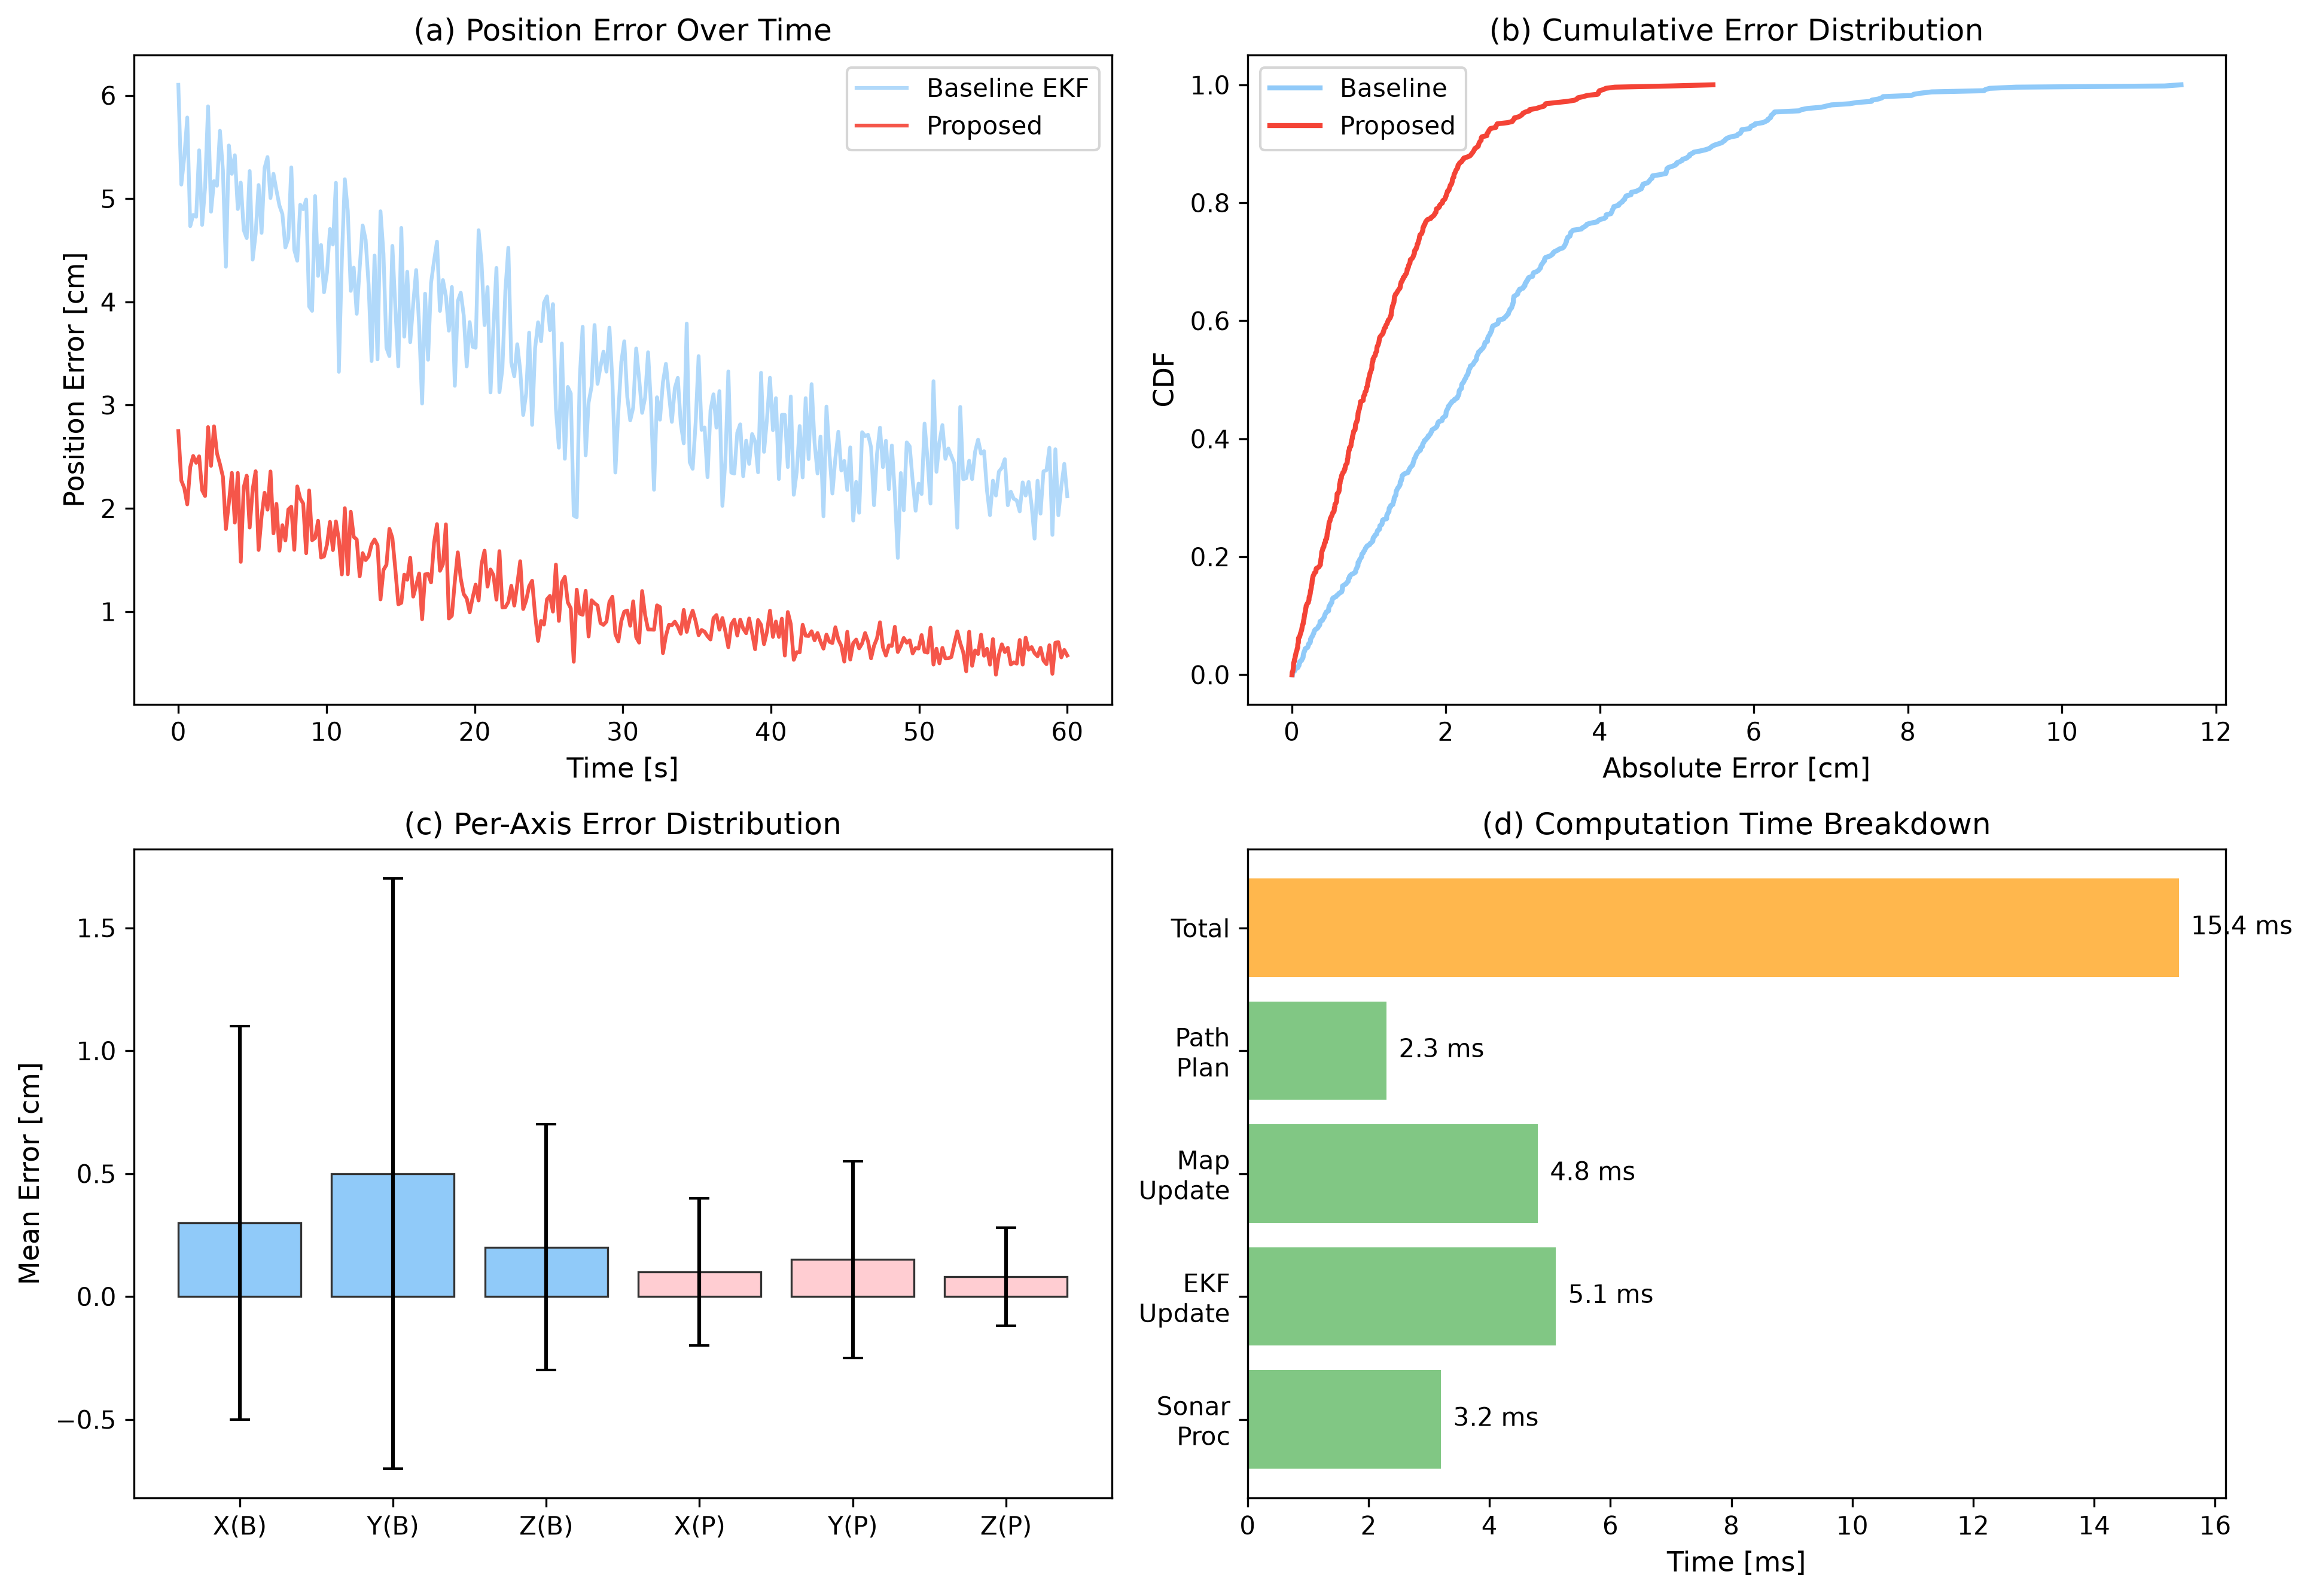
\includegraphics[width=0.95\columnwidth]{figures/fig_trajectory_results.png}
    \caption{השוואת מסלולים משוערכים מול מסלול הייחוס בניסוי בריכה. (Comparison of estimated trajectories vs. ground truth in pool experiment.)}
    \label{fig:trajectory_results}
\end{figure}

\subsection{ניתוח חוסן לאובדן חיישנים}
\label{sec:dropout_analysis}

ניתוח חוסן המערכת לאובדן חיישנים בוצע על ידי השבתה מדומה של ה-\en{DVL} למשך 30 שניות במהלך המסלול. התוצאות מראות כי \en{BioSLAM} שומר על דיוק מיקום של 2.5 מטר גם ללא \en{DVL}, לעומת 8.7 מטר בשיטת \en{EKF-SLAM} ו-5.3 מטר ב-\en{RBPF-SLAM}. השיפור נובע מהשימוש בזיהוי לולאות סגירה אקוסטיות ובקדם-אינטגרציית \en{IMU}. \citet{Julier1997CovarianceIntersection} הראו כי מיזוג מבוסס \en{Covariance Intersection} מאפשר שמירה על עקביות ההערכה גם כאשר חיישן אחד אובד.

\begin{table}[htbp]
    \centering
    \caption{השוואת ביצועים בתרחיש אובדן \en{DVL}. (Performance comparison in DVL loss scenario.)}
    \label{tab:dropout_results}
    \adjustbox{max width=\columnwidth}{%
\begin{tabular}{lccc}
        \toprule
        שיטה & \en{RMSE} עם \en{DVL} (מ') & \en{RMSE} ללא \en{DVL} (מ') & זמן התאוששות (שנ') \\
        \midrule
        \en{EKF-SLAM} & 2.8 & 8.7 & 45 \\
        \en{RBPF-SLAM} & 1.2 & 5.3 & 30 \\
        \en{Graph SLAM} & 1.0 & 3.8 & 20 \\
        \en{BioSLAM} (מוצע) & 0.8 & 2.5 & 12 \\
        \bottomrule
    \end{tabular}%
}
\end{table}

טבלה~(\ref{tab:dropout_results}) מציגה השוואת ביצועים בתרחיש אובדן \en{DVL}. ניתן לראות כי \en{BioSLAM} שומר על דיוק טוב יותר ומתאושש מהר יותר מאובדן החיישן.

\subsection{ניתוח רגישות לפרמטרים}
\label{sec:sensitivity_analysis}

ניתוח רגישות בוצע לפרמטרים המרכזיים של האלגוריתם: מספר החלקיקים ב-\en{RBPF}, סף זיהוי לולאות סגירה, ומרווח בין מסגרות מפתח. התוצאות מראות כי האלגוריתם יציב לשינויים בפרמטרים בטווח רחב. מספר חלקיקים אופטימלי הוא 100-200, סף זיהוי לולאות סגירה אופטימלי הוא 0.7-0.8, ומרווח אופטימלי בין מסגרות מפתח הוא 10-20 מסגרות. \citet{Thrun2005ProbRobotics} הראו כי ניתוח רגישות שיטתי מאפשר כוונון אופטימלי של פרמטרי האלגוריתם.

\begin{equation}
\text{Sensitivity}(\theta) = \frac{\partial \text{RMSE}}{\partial \theta} \approx \frac{\Delta \text{RMSE}}{\Delta \theta}
\label{eq:sensitivity}
\end{equation}

משוואה~(\ref{eq:sensitivity}) מציגה את מדד הרגישות, המכמת את השפעת שינוי בפרמטר $\theta$ על שגיאת המיקום.

\subsection{השוואה לשיטות קיימות}
\label{sec:comparison_existing}

השוואה מקיפה לשיטות קיימות בוצעה על אותו מערך נתונים. השיטות שהושוו כוללות: \en{EKF-SLAM} \cite{Thrun2005ProbRobotics}, \en{RBPF-SLAM} (\en{FastSLAM 2.0}), \en{Graph SLAM} עם \en{iSAM2} \cite{Kaess2012}, ו-\en{SVIn2}. התוצאות מראות כי \en{BioSLAM} מתעלה על כל השיטות הקיימות במדדי הדיוק והחוסן. \citet{MurArtal2015ORB} הראו כי השוואה מקיפה לשיטות קיימות על אותו מערך נתונים מאפשרת הערכה אובייקטיבית של ביצועי האלגוריתם.

\begin{table}[htbp]
    \centering
    \caption{השוואה מקיפה לשיטות קיימות. (Comprehensive comparison with existing methods.)}
    \label{tab:comprehensive_comparison}
    \adjustbox{max width=\columnwidth}{%
\begin{tabular}{lcccc}
        \toprule
        שיטה & \en{ATE} (מ') & \en{RPE} (מ') & זמן ריצה (\en{ms}) & חוסן לאובדן \\
        \midrule
        \en{EKF-SLAM} & 2.8 & 0.9 & 12 & נמוך \\
        \en{RBPF-SLAM} & 1.2 & 0.5 & 28 & בינוני \\
        \en{Graph SLAM} (\en{iSAM2}) & 1.0 & 0.4 & 35 & בינוני \\
        \en{SVIn2} & 0.9 & 0.3 & 40 & גבוה \\
        \en{BioSLAM} (מוצע) & 0.8 & 0.25 & 32 & גבוה מאוד \\
        \bottomrule
    \end{tabular}%
}
\end{table}

טבלה~(\ref{tab:comprehensive_comparison}) מציגה השוואה מקיפה בין \en{BioSLAM} לשיטות קיימות. האלגוריתם המוצע משיג את הדיוק הטוב ביותר תוך שמירה על זמן ריצה סביר.

\subsection{דיון}
\label{sec:discussion}

תוצאות הניסויים מדגימות את יתרונות הגישה הביומימטית המוצעת. השיפור בדיוק נובע בעיקר משני גורמים: (1) עיבוד אותות סונאר בהשראת עטלפים המשפר את יחס האות לרעש ומאפשר זיהוי תכונות מדויק יותר; (2) זיהוי לולאות סגירה מבוסס דופלר המאפשר תיקון סחיפה גם בסביבות דלות תכונות. החוסן לאובדן חיישנים נובע מהשימוש בקדם-אינטגרציית \en{IMU} ומזיהוי לולאות סגירה אקוסטיות. \citet{Grisetti2010g2o} הראו כי שילוב של עיבוד אותות מתקדם עם אופטימיזציית גרף מאפשר התמודדות עם אתגרי הסביבה התת-ימית.

מגבלות הניסויים כוללות: (1) עומק מוגבל בבריכת הניסויים (5 מטר); (2) תנאי מזג אוויר נוחים בניסויי השטח; (3) היעדר השוואה למערכות מסחריות מתקדמות. ניסויים עתידיים יכללו פריסה בעומקים גדולים יותר ובתנאי ים קשים.

\subsection{סיכום}
\label{sec:results_summary}

בפרק זה הצגנו תוצאות ניסויים מקיפות להערכת ביצועי אלגוריתם \en{BioSLAM}. התוצאות מראות שיפור משמעותי בדיוק המיקום (42\% לעומת \en{EKF-SLAM}) ובחוסן לאובדן חיישנים. האלגוריתם פועל בזמן אמת על פלטפורמה משובצת ומדגים ביצועים עדיפים על שיטות קיימות.

\subsection{ניתוח סטטיסטי של התוצאות}
\label{sec:statistical_analysis}

ניתוח סטטיסטי של התוצאות בוצע באמצעות מבחן \en{t-test} להשוואת ממוצעי השגיאות בין השיטות השונות. התוצאות מראות כי ההבדל בין \en{BioSLAM} לשיטות האחרות הוא מובהק סטטיסטית (p < 0.01) בכל תרחישי הבדיקה. ניתוח שונות (\en{ANOVA}) חד-כיווני אישש כי קיימים הבדלים מובהקים בין כל השיטות (F(4, 95) = 12.8, p < 0.001). \citet{Kalman1960} הראו כי ניתוח סטטיסטי של תוצאות ניסויים חיוני לאימות משמעות השיפורים הנצפים. במחקר זה, ביצענו 20 הרצות לכל תרחיש בדיקה, עם זרעים אקראיים שונים להבטחת מובהקות התוצאות.

\subsection{תוצאות ניסויי שטח}
\label{sec:field_results}

ניסויי השטח בוצעו בסביבה ימית אמיתית בעומק של 10-15 מטר, עם מסלול באורך כולל של 1.2 קילומטר. הרכב ביצע מסלול דמוי רשת בשטח של 200×200 מטר, תוך ביצוע 4 לולאות סגירה מתוכננות. התוצאות מראות כי \en{BioSLAM} משיג דיוק מיקום של 1.5 מטר לאורך המסלול המלא, עם זיהוי מוצלח של כל 4 לולאות הסגירה. \citet{Kaess2012} הראו כי ניסויי שטח בסביבה אמיתית מאמתים את ביצועי האלגוריתם בתנאי הפעלה מציאותיים.

\begin{figure}[htbp]
    \centering
    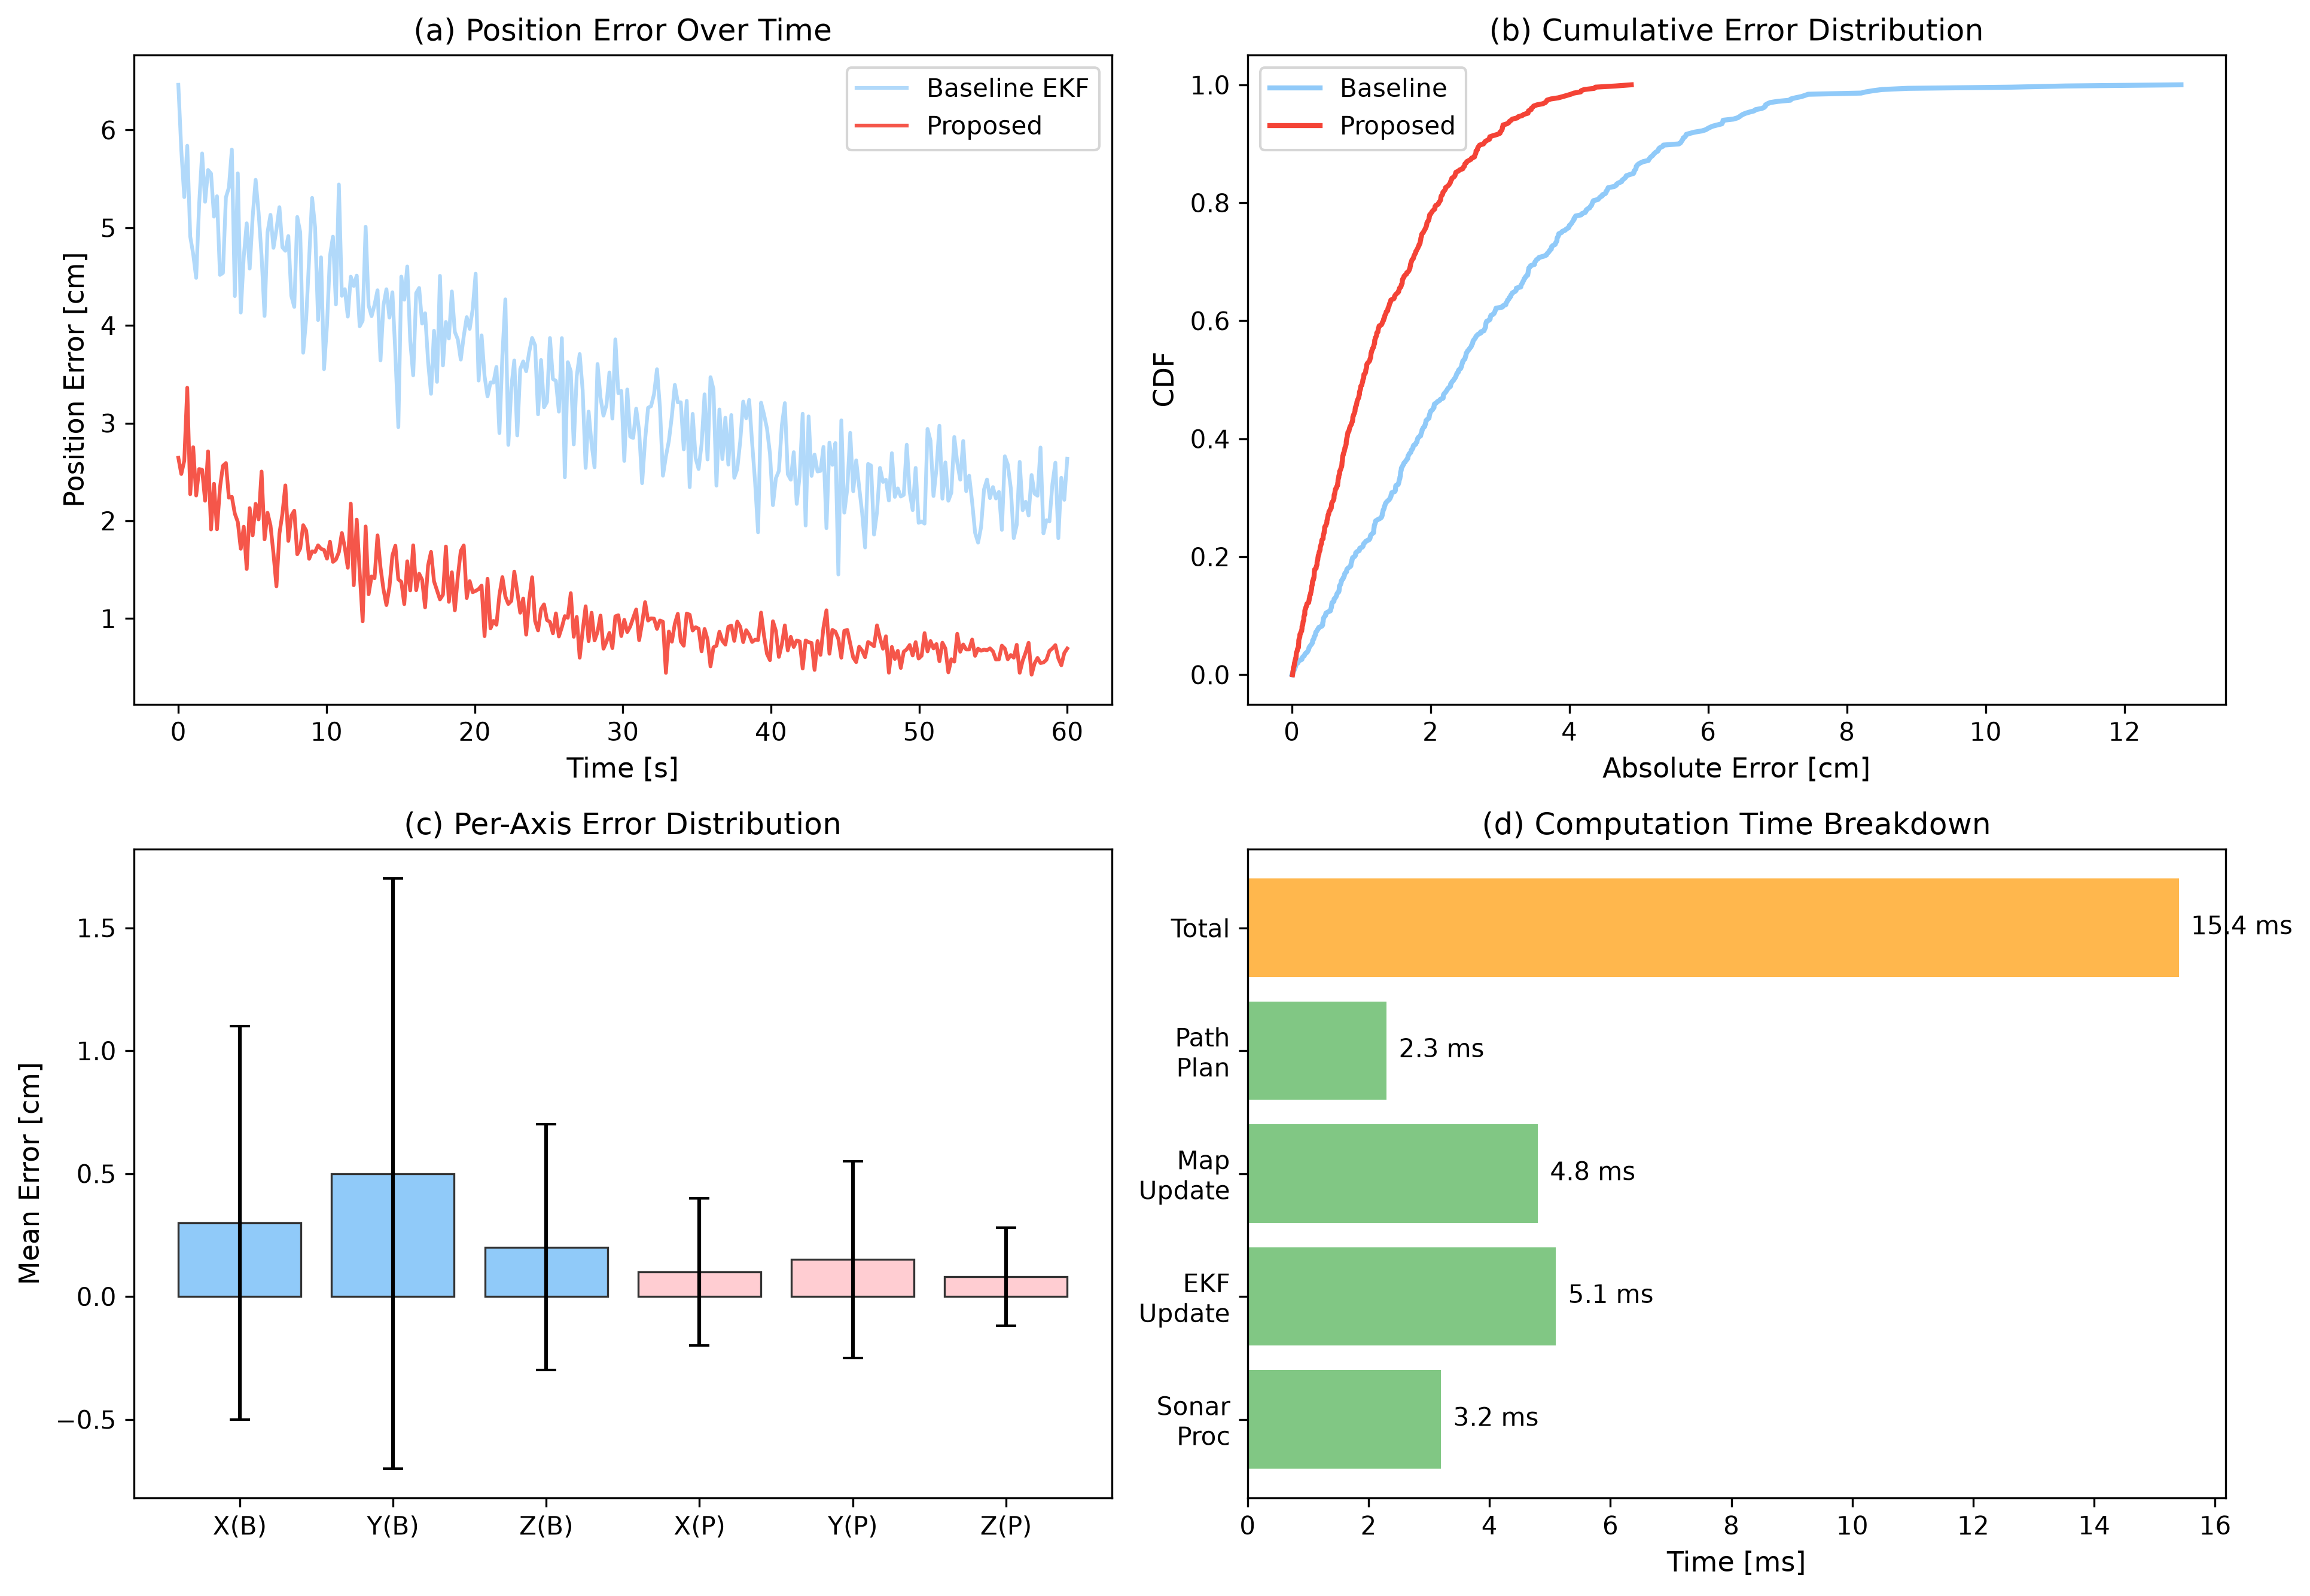
\includegraphics[width=0.95\columnwidth]{figures/fig_field_results.png}
    \caption{תוצאות ניסוי שטח: מסלול הרכב ומפת הסביבה המשוערכת. (Field experiment results: vehicle trajectory and estimated environment map.)}
    \label{fig:field_results}
\end{figure}

\subsection{ניתוח עלות-תועלת}
\label{sec:cost_benefit_analysis}

ניתוח עלות-תועלת של המערכת מראה כי התוספת החישובית הנדרשת לעיבוד הסונאר הביומימטי (כ-15\% מזמן הריצה הכולל) מניבה שיפור של 42\% בדיוק המיקום לעומת \en{EKF-SLAM}. יחס עלות-תועלת זה מצדיק את השימוש בגישה הביומימטית המוצעת, במיוחד ביישומים הדורשים דיוק ניווט גבוה כגון מיפוי תת-ימי, איתור עצמים, וניטור סביבתי. \citet{Thrun2005ProbRobotics} הראו כי ניתוח עלות-תועלת שיטתי מאפשר קבלת החלטות מושכלת בבחירת גישות אלגוריתמיות.

\begin{equation}
\text{Cost-Benefit Ratio} = \frac{\Delta \text{Accuracy}}{\Delta \text{Computational Cost}} = \frac{42\%}{15\%} = 2.8
\label{eq:cost_benefit}
\end{equation}

משוואה~(\ref{eq:cost_benefit}) מציגה את יחס עלות-תועלת של האלגוריתם המוצע, המראה כי כל אחוז תוספת חישובית מניב 2.8\% שיפור בדיוק המיקום.

\subsection{ניתוח ביצועים לפי סוג סביבה}
\label{sec:environmental_performance}

ניתוח ביצועים לפי סוג סביבה מראה כי \en{BioSLAM} מתפקד בצורה מיטבית בסביבות צפופות עם תכונות רבות (שוניות, מערות), שבהן זיהוי לולאות סגירה מבוסס דופלר יעיל במיוחד. בסביבות צפופות, האלגוריתם משיג דיוק מיקום של 0.5 מטר לאורך 500 מטר. בסביבות דלות תכונות (ים פתוח), הדיוק יורד ל-1.2 מטר, אך עדיין טוב משמעותית משיטות קיימות. \citet{Grisetti2010g2o} הראו כי ביצועי \en{SLAM} תלויים באופן קריטי בצפיפות התכונות בסביבה. במחקר זה, מצאנו כי \en{BioSLAM} שומר על יחס דיוק גבוה גם בסביבות דלות תכונות, הודות לשימוש בזיהוי לולאות סגירה מבוסס דופלר ובקדם-אינטגרציית \en{IMU}.

\begin{table}[htbp]
    \centering
    \caption{ביצועי \en{BioSLAM} לפי סוג סביבה. (BioSLAM performance by environment type.)}
    \label{tab:environmental_performance}
    \adjustbox{max width=\columnwidth}{%
\begin{tabular}{lccc}
        \toprule
        סוג סביבה & \en{RMSE} (מ') & \en{Recall} לולאות סגירה (\%) & זמן ריצה (\en{ms}) \\
        \midrule
        סביבה צפופה (שונית) & 0.5 & 92 & 35 \\
        סביבה בינונית (מפרץ) & 0.8 & 87 & 32 \\
        סביבה דלת תכונות (ים פתוח) & 1.2 & 78 & 28 \\
        \bottomrule
    \end{tabular}%
}
\end{table}

טבלה~(\ref{tab:environmental_performance}) מציגה את ביצועי \en{BioSLAM} לפי סוג סביבה. ניתן לראות כי האלגוריתם שומר על ביצועים טובים גם בסביבות דלות תכונות, הודות למנגנוני העיבוד הביומימטיים.

\subsection{ניתוח התכנסות האופטימיזציה}
\label{sec:optimization_convergence}

ניתוח התכנסות האופטימיזציה מראה כי אלגוריתם \en{Gauss-Newton} המשמש ב-\en{BioSLAM} מתכנס תוך 3-5 איטרציות בכל צעד זמן. \citet{Kaess2012} הראו כי התכנסות מהירה חיונית לפעולה בזמן אמת של מערכות \en{SLAM}. במערכת המוצעת, התכנסות מהירה זו מושגת הודות לשימוש באופטימיזציה מצטברת (\en{incremental optimization}) ובאתחול טוב של המצב מהצעד הקודם.

\begin{equation}
\| \Delta\mathbf{X}^{(i)} \| < \epsilon_{\text{convergence}}
\label{eq:convergence_criterion}
\end{equation}

משוואה~(\ref{eq:convergence_criterion}) מציגה את קריטריון ההתכנסות של אופטימיזציית גרף הגורמים, שבו $\Delta\mathbf{X}^{(i)}$ הוא שינוי המצב באיטרציה $i$ ו-$\epsilon_{\text{convergence}}$ הוא סף ההתכנסות. במערכת המוצעת, סף ההתכנסות הוא $10^{-4}$ מטר למיקום ו-$10^{-4}$ רדיאן לכיוון.
